\chapter{Einleitung}

Im folgenden Abschnitt werden die aus technischer Sicht relevanten Aspekte genauer analysiert. Zu Beginn wird das Aufgabenumfeld in einem weiteren Sinne betrachtet, und die Kernelemente der Applikation aufgezeigt. Danach wird auf die Analyse und die Realisierung eingegangen. Der Hauptteil richtet sich vor allem an Entwickler, die an der Weiterentwicklung des Produktes interessiert sind.

\section{Big Picture}

Zur Übersicht werden die verschiedenen Komponenten des Projektes in einem Big Picture zusammengefasst.
Die Darstellung ist in drei Abschnitte unterteilt. Im obersten Abschnitt befinden sich alle Geräte, welche Daten sammeln und diese zur Verfügung stellen. Diese Aufnahmesysteme bestehen aus der Android TourLiveApp, als Teil dieser Arbeit, sowie dem Android RadioTourSpeaker welcher im Rahmen einer anderen Arbeit entwickelt wurde. \\
Im mittleren Teil befinden sich die Serversysteme. Diese besteht aus einem TourLiveServer, welcher die Renndaten empfängt und verarbeitet sowie dem Geräteverwaltungsserver. Der Geräteverwaltungsserver bietet eine Übersicht über die registrierten Aufnahmesysteme und ermöglicht es deren Einstellungen zu Verwalten sowie allfällige Fehlerquellen früehzeitig zu erkennen.\\
Der unterste Abschnitt zeigt die Anwendergruppen, die mit den Daten beliefert werden. Dies kann die Webseite sein, die in dieser Arbeit umgesetzt wird, jedoch auch Drittanbieter, die Interesse an diesen Daten haben.\\
\\
Teil dieser Arbeit sind die farblich hervorgehobenen Komponenten: Die Aufnahmesysteme «TourLiveApp» in Form einer Android App [rot], das Serversystem «TourLiveServer» in Form eines Spring Webservices [blau] sowie das Serversystem «TourLiveDeviceManagementServer» ebenfalls in Form eines Spring Webservices [grün].

\begin{figure}[H]
	\caption{BigPicture}
	\centering
	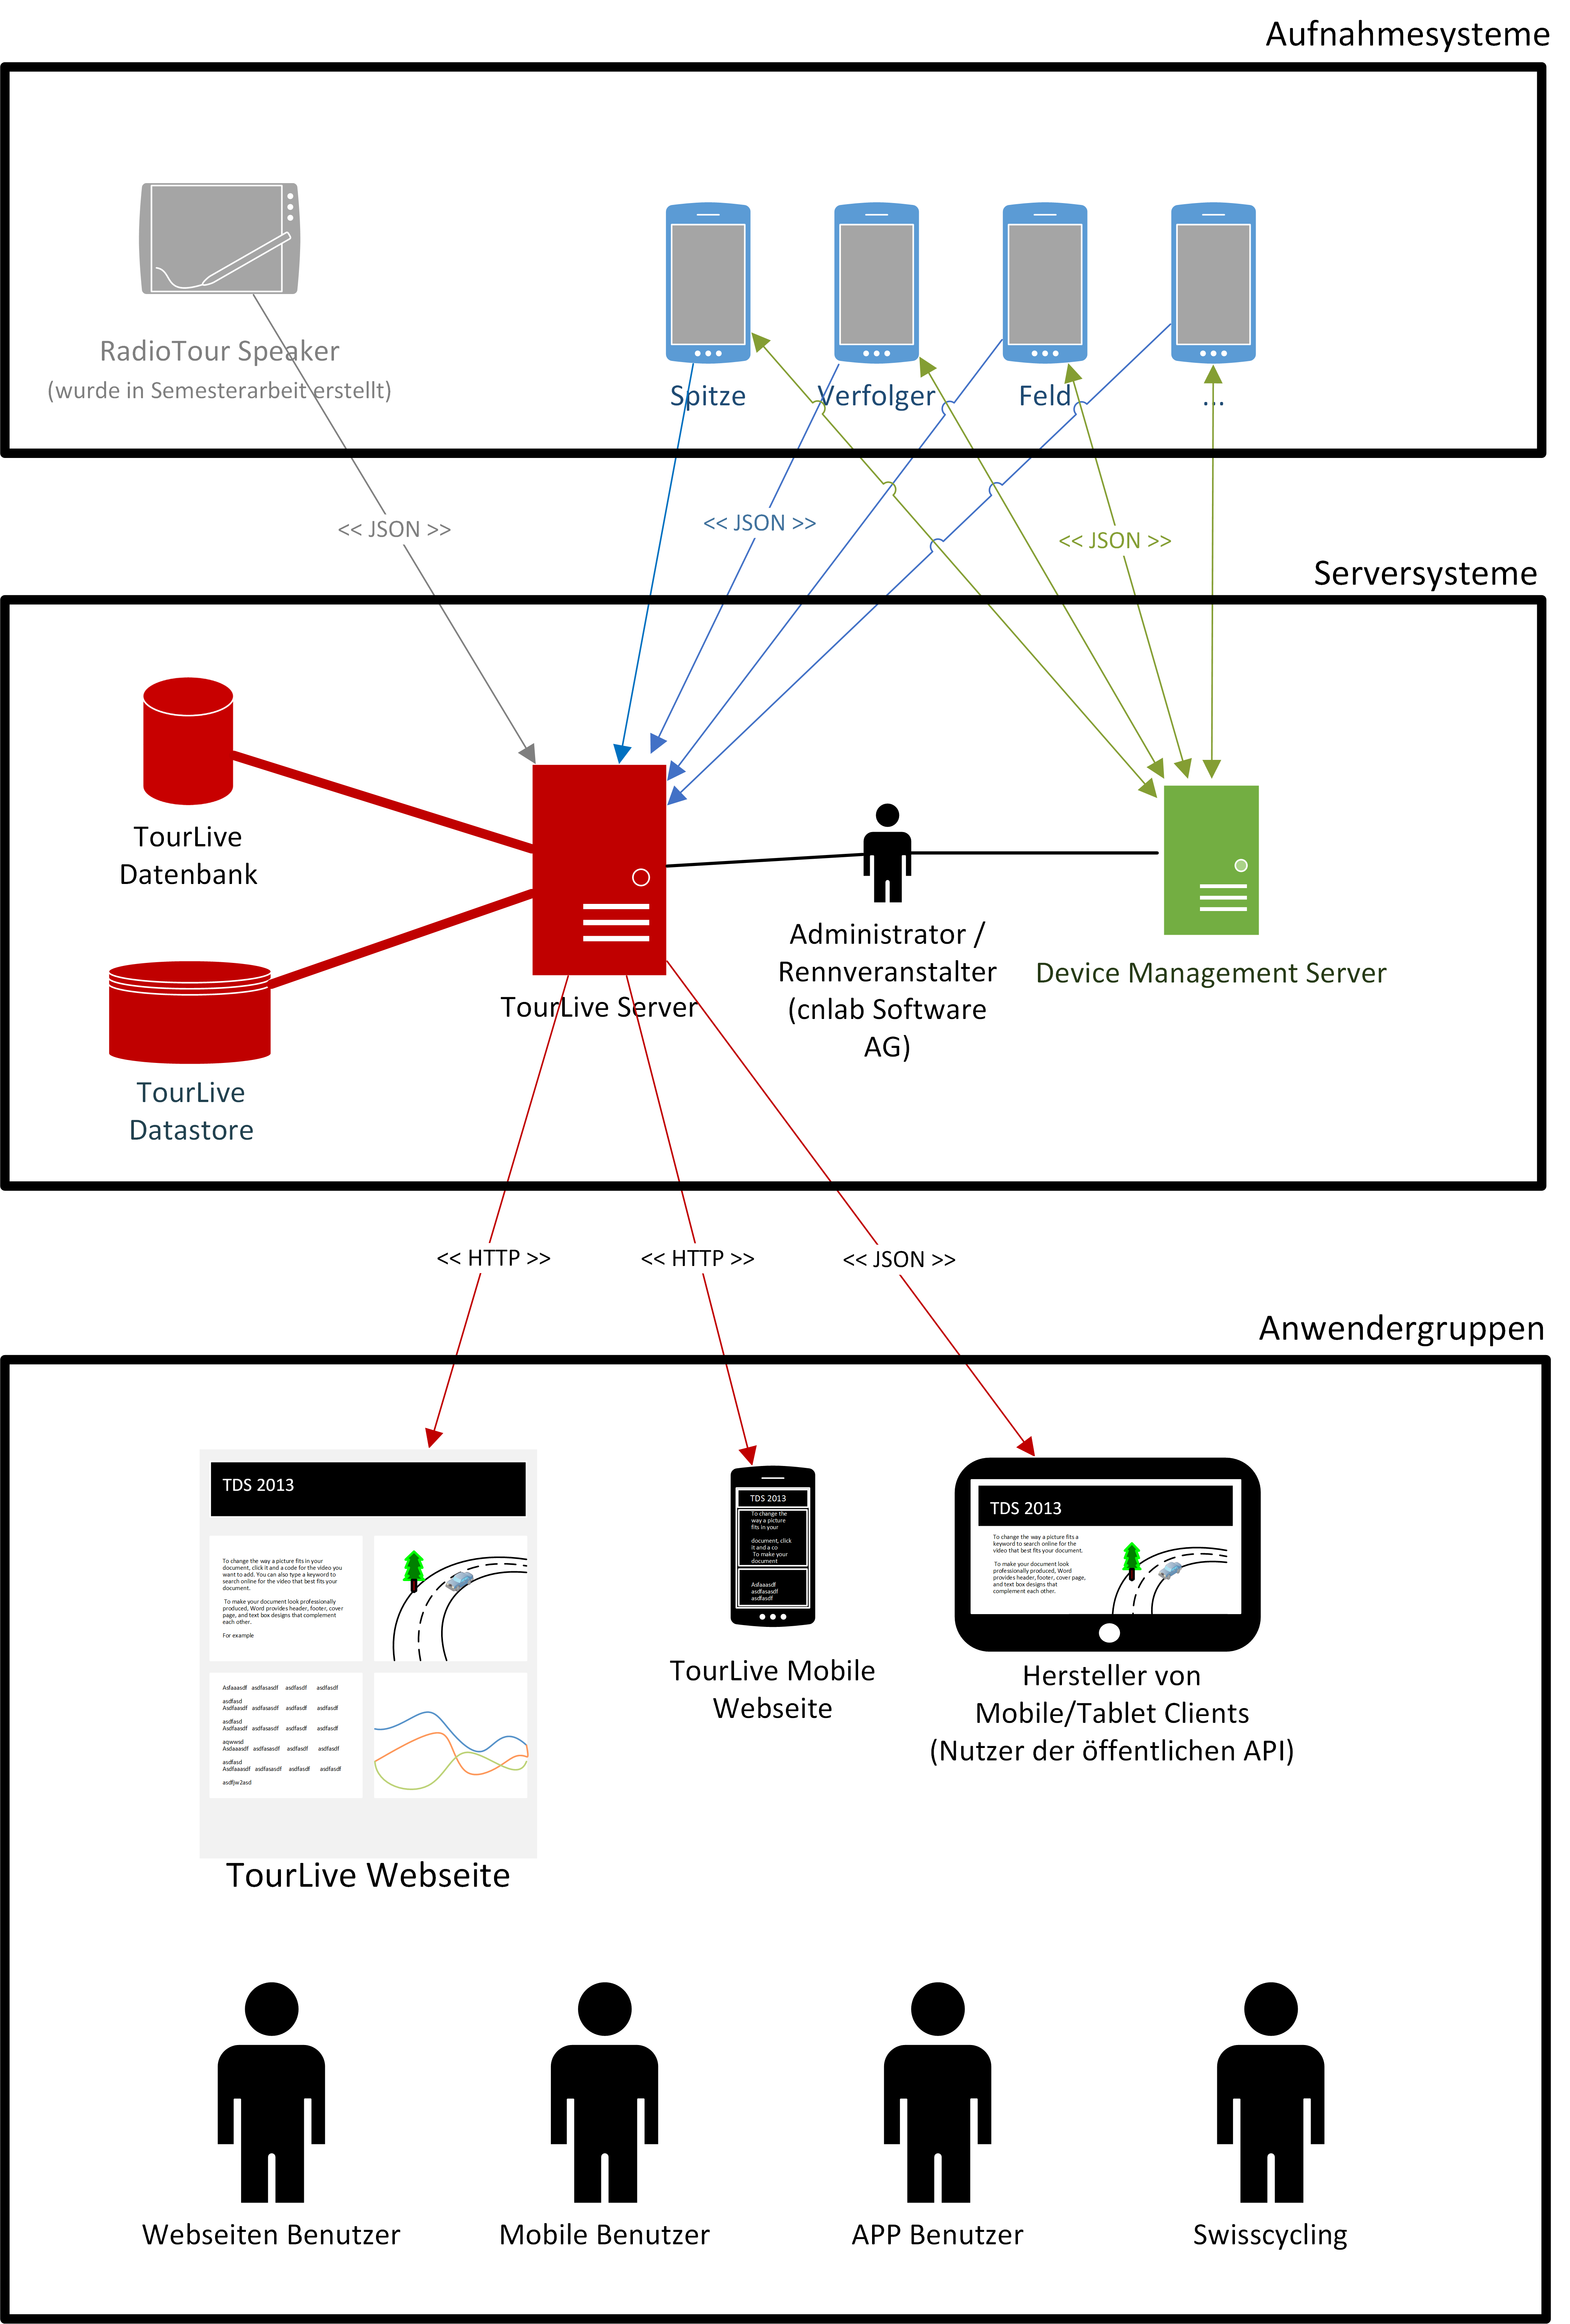
\includegraphics[height=200mm]{images/BigPicture.png}
\end{figure}

\pagebreak

\section{Aufgabenteilung}

{\renewcommand{\arraystretch}{2}%
    \begin{longtable}{  p{9.0cm} | p{3.0cm} }

    \textbf{Aufgabe} & \textbf{Erledigt durch} \\ 
  	\hline
	\hline
    TourLiveServer & Florian Bentele \\
    \hline
    TourLiveApp & Patrizia Heer Simon Stäheli \\
    \hline
    TourLiveDeviceManagementServer & Patrizia Heer Simon Stäheli \\
    \hline

\caption{Aufgabenteilung}
\end{longtable}}
